\documentclass[../../main.tex]{subfiles}
\begin{document}

\begin{flushright}
\footnotesize\textit{【自動文字起こし・要確認】}
\end{flushright}

{\bf [解]}
$P$から引いた接線が座標軸に平行になる時，(i)から$P$の$x$座標が$\pm\dfrac{1}{\sqrt3}$である．このうち(i)を満たすのは$P$の$y$座標が$|y|\le1$をみたす時．以下，他の場合を考える．

この時$P$から引いた接線$\ell$として
\begin{align*}
\ell: y=m(x-a)+b
\end{align*}
とおける．$m\in\mathbb{R}$，$P(a,b)$とした．$\cdots\bigstar$

ここで，$X=\sqrt3x,\ Y=y$なる変換を考える．この変換によって図形$A$が$A'$にうつると表す．楕円は$X^2+Y^2=1$に，$\ell$は$\ell'$にうつり，$\ell'$と円$X^2+Y^2=1$は接している．
\begin{align*}
\ell': Y=m\left(\frac{1}{\sqrt3}X-a\right)+b
\end{align*}
で接する条件から
\begin{align*}
\frac{|-am+b|}{\sqrt{\frac13m^2+1}}=1
\end{align*}
両辺0以上から2乗しても良く，
\begin{align*}
\left(a^2-\frac13\right)m^2-2abm+b^2-1=0 \quad\cdots\text{①}
\end{align*}
$m$の2次方程式①の2実解$m_1,m_2\ (m_1\le m_2)$とする．
\begin{align*}
\text{①の判別式}D\text{として，}\quad\frac{D}{4}=a^2b^2-\left(a^2-\frac13\right)(b^2-1)=a^2+\frac13b^2-\frac13\ge0
\end{align*}
又，$a\ne\dfrac{1}{\sqrt3}$から①は2次式．

まず，条件(i)を考える．(i)がみたされる時，$A\left(\dfrac{1}{\sqrt3},0\right)$として，線分$AP$上の点$B(t(a-\tfrac{1}{\sqrt3})+\tfrac{1}{\sqrt3},\ tb)\ (0\le t\le1)$と楕円の共有点が$A$のみであるから，
\begin{align*}
3\left\{t\left(a-\frac{1}{\sqrt3}\right)+\frac{1}{\sqrt3}\right\}^2+t^2b^2=1
\end{align*}
\begin{align*}
\left\{3\left(a-\frac{1}{\sqrt3}\right)^2+b^2\right\}t^2+2\sqrt3\left(a-\frac{1}{\sqrt3}\right)t=0
\end{align*}
の$t\ne0$の解が負ならば良く，
\begin{align*}
a-\frac{1}{\sqrt3}\ge0 \iff a\ge\frac{1}{\sqrt3} \quad\cdots\text{②}
\end{align*}

次に，条件(ii)をかんがえる．$\angle QPR\ge\angle R$の時，$\overrightarrow{PQ}\cdot\overrightarrow{PR}\le0$である．
\begin{align*}
\begin{pmatrix}-1\\m_1\end{pmatrix}\cdot\begin{pmatrix}-1\\m_2\end{pmatrix}\le0 \quad\therefore\ 1+m_1m_2\le0
\end{align*}
①の$m_1m_2=(b^2-1)/(a^2-\tfrac13)$だから，代入して
\begin{align*}
1\le\frac{1-b^2}{a^2-\frac13}
\end{align*}
②から，$a^2-\dfrac13\ge0$だから
\begin{align*}
a^2-\frac13\le1-b^2 \quad\therefore\ a^2+b^2\le\frac43 \quad\cdots\text{③}
\end{align*}
②③と前半の議論により図示するのは下図斜線部（境界含む）で，面積$S$として
\begin{align*}
S=\frac12\cdot\frac{2\pi}{3}\cdot\frac43-\frac{\sqrt3}{3}
\end{align*}
\begin{align*}
=\frac13\left(\frac{4}{3}\pi-\sqrt3\right)
\end{align*}

\begin{figure}[htb]
\begin{center}
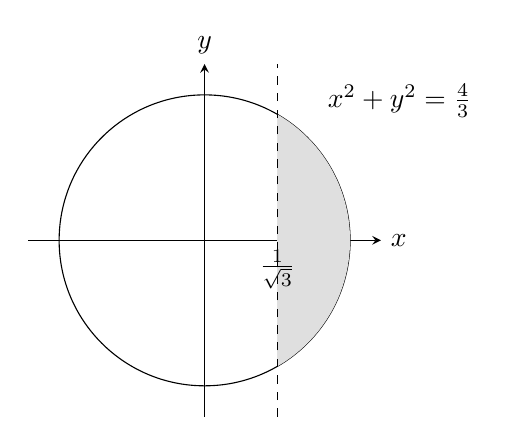
\begin{tikzpicture}[scale=1.6, >=stealth]
  \draw[->] (-1.4,0) -- (1.4,0) node[right] {$x$};
  \draw[->] (0,-1.4) -- (0,1.4) node[above] {$y$};
  \draw (0,0) circle (1.1547);
  \begin{scope}
    \clip (0,0) circle (1.1547);
    \fill[gray!25] (0.5774,-1.4) rectangle (1.4,1.4);
  \end{scope}
  \draw[dashed] (0.5774,-1.4) -- (0.5774,1.4);
  \node[below] at (0.5774,0) {$\frac{1}{\sqrt3}$};
  \node[above right] at (0.9,0.9) {$x^2+y^2=\frac43$};
\end{tikzpicture}
\end{center}
\caption{面積$S$を求める領域の図示（斜線部）}
\end{figure}


\end{document}
